\section{Volatage Regulator using LM2596}
LM2596 is a voltage regulator mainly used to step down the voltage or to drive load under
3A. It is also known as DC-to-DC power converter or buck converter which is used to step
down the voltage from its input supply to the output load. The current goes up during this
voltage step down process.

LM2596 comes with a remarkable load and line regulation. It is available in both versions:
fixed output voltage version with 3.3V, 5V, 12V, and customized output version where you
can choose the output as per your requirement. This regulator is incorporated with a
fixed-frequency oscillator and an internal frequency compensation method.

The typical connection for LM2596 is proposed by Texas Instrument (TI), as following:

\begin{figure}[ht]
    \centering
    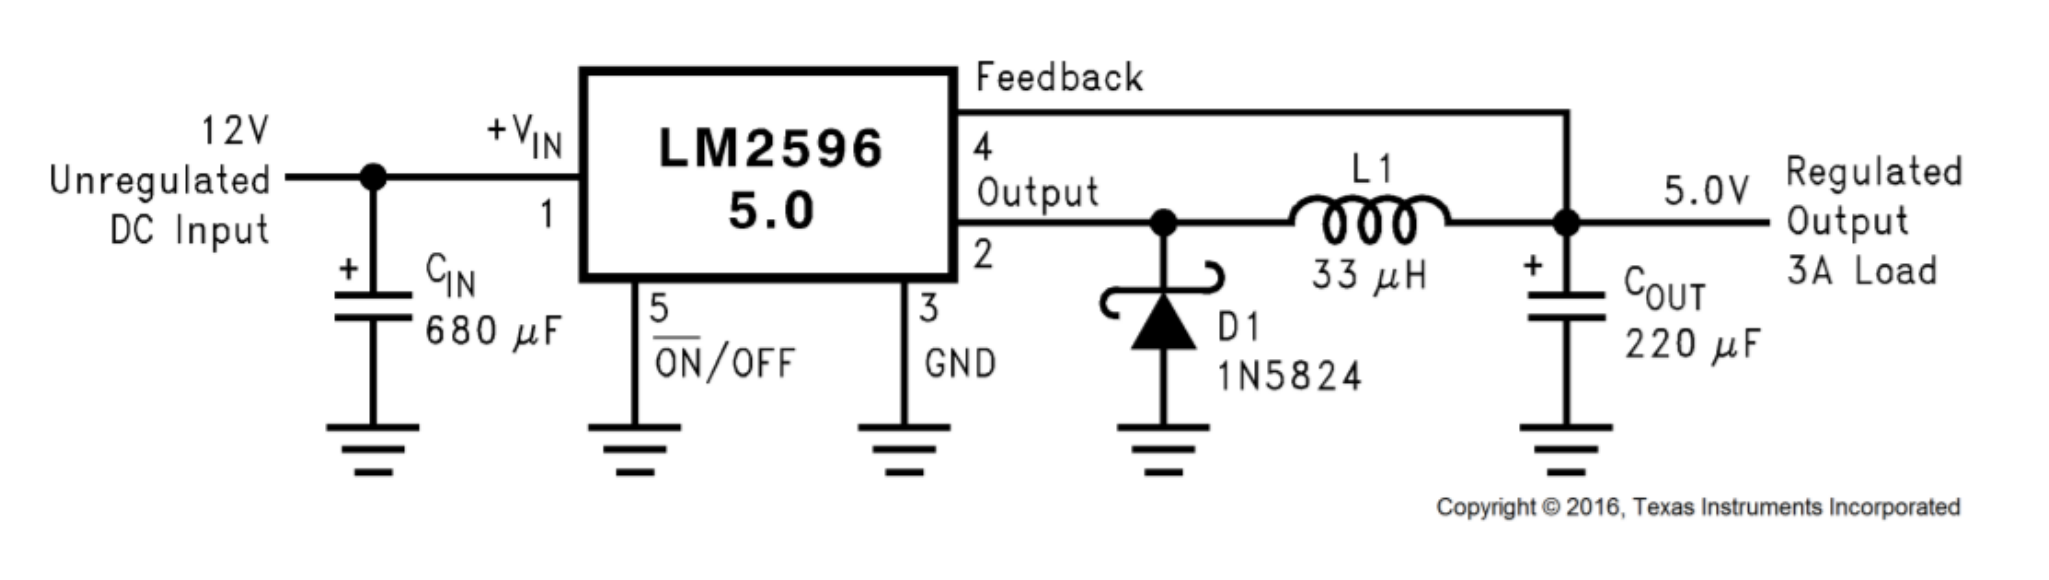
\includegraphics[scale=0.25]{graphics/ex2/f1.png}
    \caption{Typical connection for LM2596}
\end{figure}

\subsection{Schematic design}
Students are proposed to capture the schematic design in Altium Designer and place the
image in this part.

Some hot keys are normally used in the schematic is the space bar, X( horizontal mirror),
Y (vertial mirror) and Ctrl + W (place a wire).

\pagebreak

\textbf{Your image goes here}

\begin{figure}[ht]
    \centering
    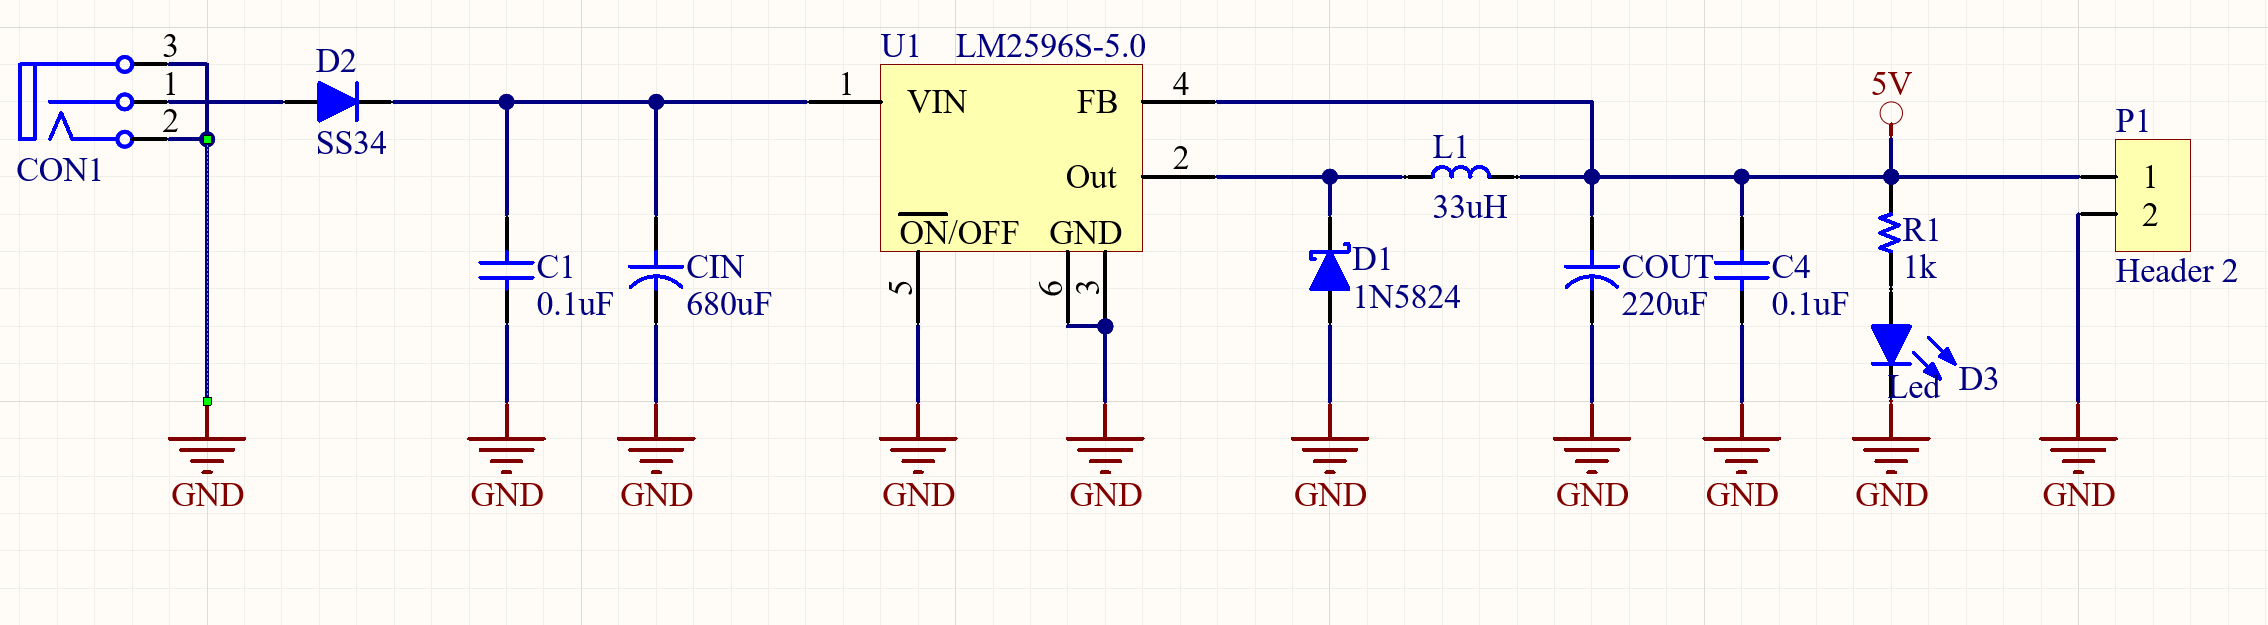
\includegraphics[scale=0.26]{graphics/ex2/f3.png}
    \caption{Schematic Volatage Regulator using LM2596}
\end{figure}

\subsection{PCB layout}

Similarly to the schematic, some snap shorts of for the TOP, BOTTOM layers are required
in this report. Moreover, several 3D images of your schematic are also required.

\textbf{Your image goes here}

\begin{figure}[ht]
    \centering
    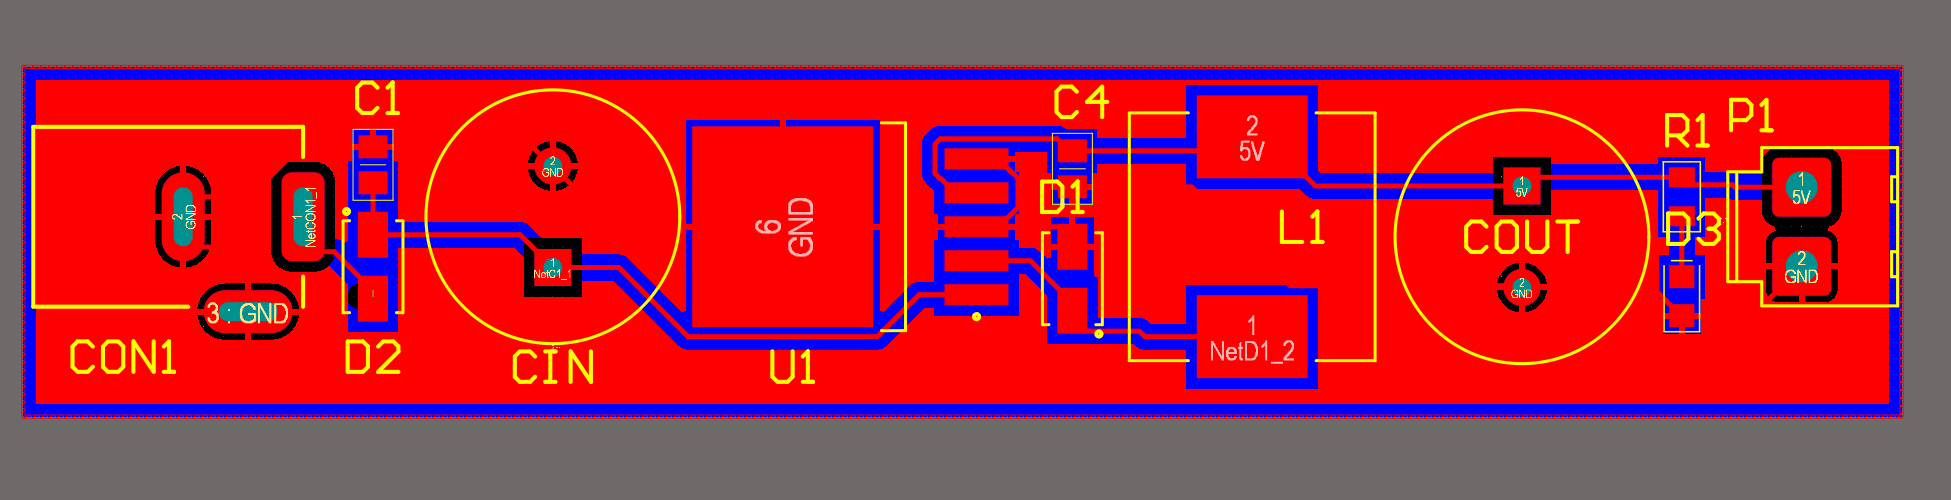
\includegraphics[scale=0.3]{graphics/ex2/f4.png}
    \caption{TOP layer}
\end{figure}

\begin{figure}[ht]
    \centering
    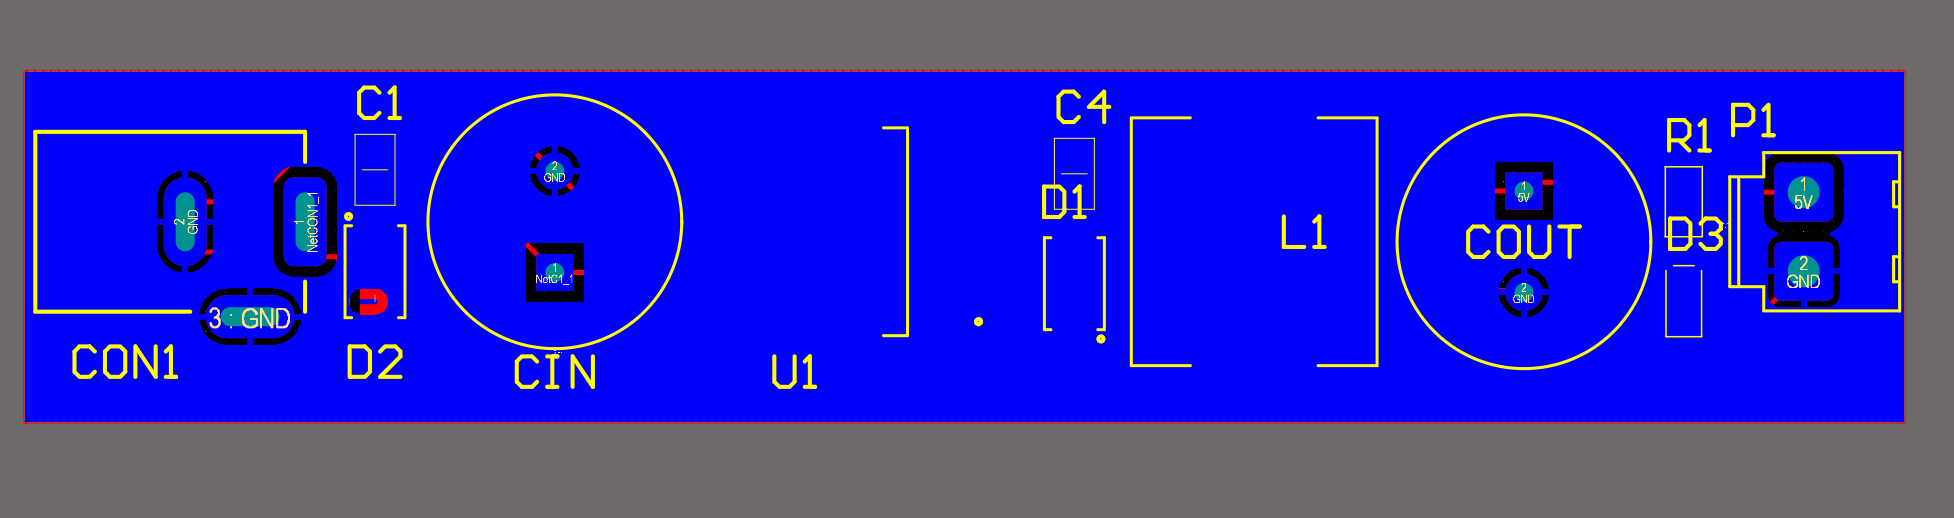
\includegraphics[scale=0.3]{graphics/ex2/f5.png}
    \caption{BOTTOM layer}
\end{figure}

\begin{figure}[ht]
    \centering
    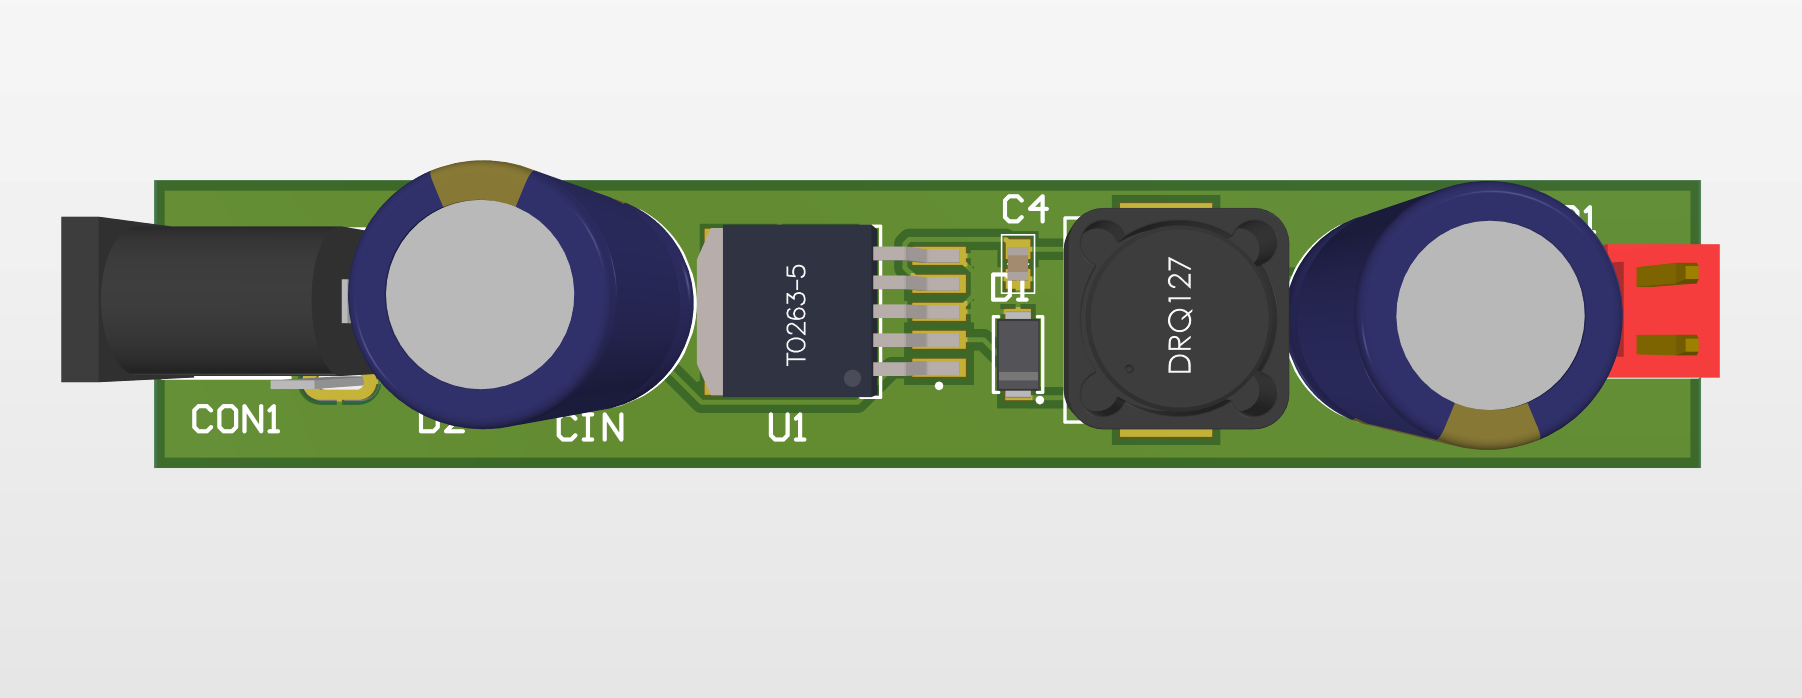
\includegraphics[scale=0.3]{graphics/ex2/f2.png}
    \caption{3D image Top view}
\end{figure}

\begin{figure}[ht]
    \centering
    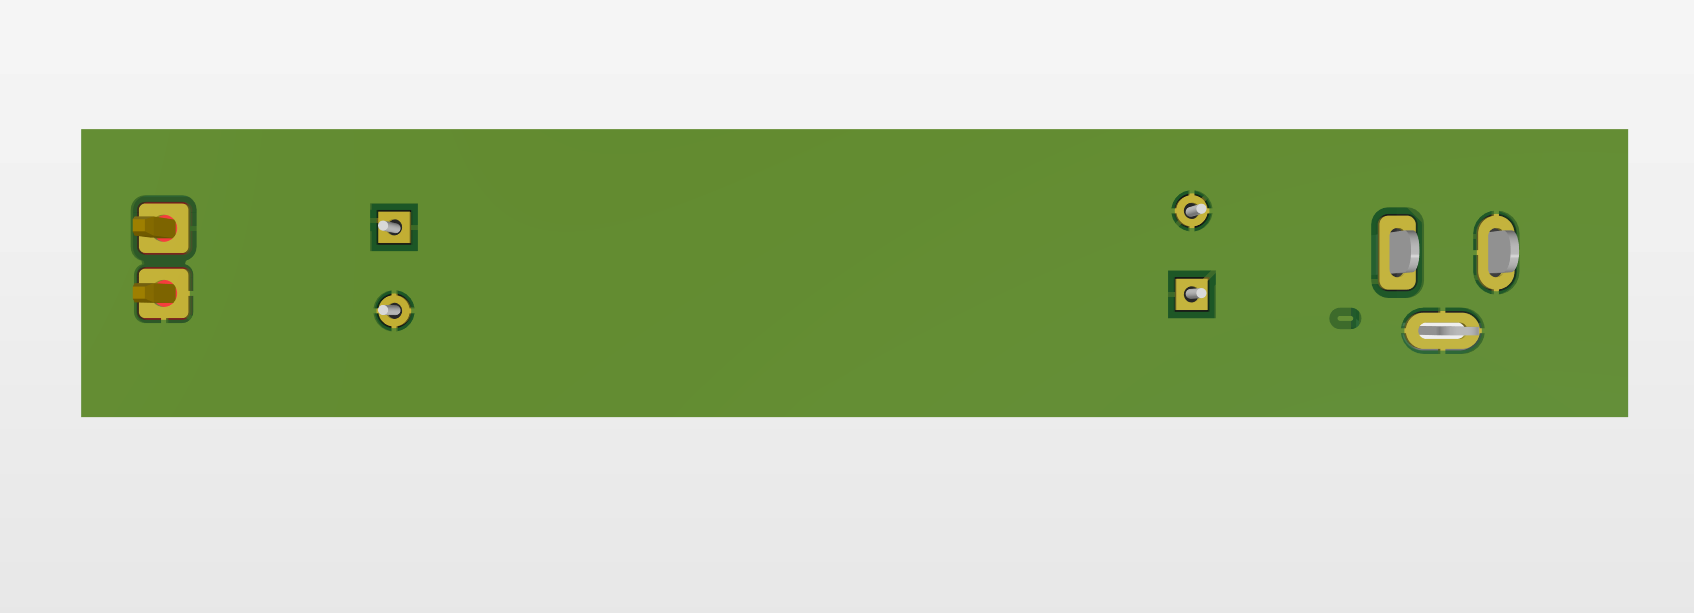
\includegraphics[scale=0.32]{graphics/ex2/f6.png}
    \caption{3D image Bottom view}
\end{figure}

\begin{figure}[ht]
    \centering
    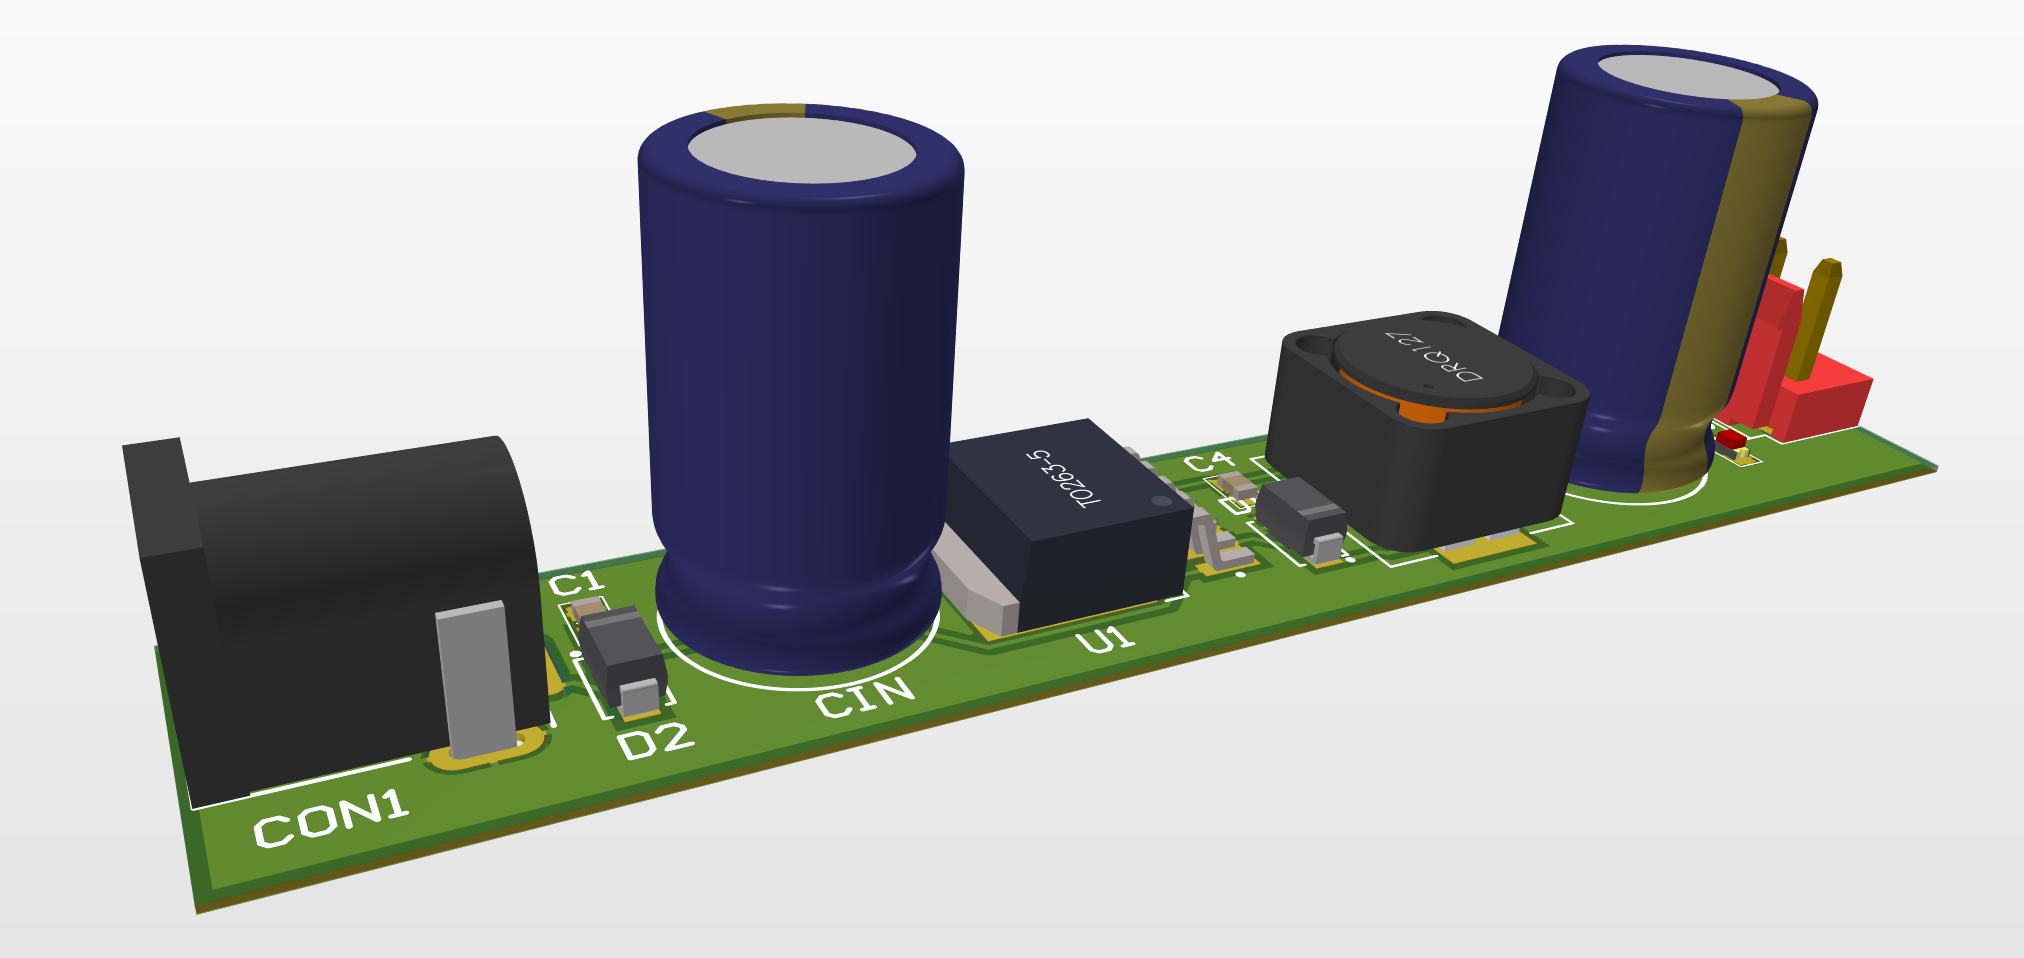
\includegraphics[scale=0.26]{graphics/ex2/f7.png}
    \caption{3D image Beside view}
\end{figure}
